\section{Application: mapping the lunar south pole}
\label{sec:southpole}

As a transfer test, the trained pipelines are deployed on the lunar south pole --- a region of high scientific and operational interest (permanently shadowed terrain, Artemis-era landing candidates) that is geologically distinct from the volcanic Marius Hills training domain. South pole imagery was obtained from the same LRO WAC source and tiled identically, producing 3\,639 tiles. No feature catalogue exists for this region, so no ground-truth masks are available: everything in this section is a transfer \emph{diagnostic} (prediction-confidence statistics), not an accuracy measurement (Sect.~\ref{sec:metrics_protocol}).

\subsection{Semantic segmentation transfer}
\label{sec:sp_unet}

Each tile is preprocessed with the same CLAHE + Sobel three-channel pipeline used in training and passed through the definitive SmallUNet checkpoint; per-class probability maps are saved as compressed \texttt{.npz} files for downstream aggregation. Table~\ref{tab:south_pole_stats} reports the aggregated statistics.

\begin{table}[htbp]
\centering
\caption{SmallUNet south pole inference (3\,639 tiles). Avg.\ Max.\ Prob.\ is the mean, over tiles, of the maximum predicted probability for each class. Global Max is the highest probability observed in any single tile.}
\label{tab:south_pole_stats}
\resizebox{\columnwidth}{!}{%
\begin{tabular}{lrrr}
\toprule
Class & Avg.\ Max.\ Prob. & Global Max & Status \\
\midrule
\texttt{impact\_crater}       & 0.863 & 1.000 & $\checkmark$ detected \\
\texttt{lobate\_scarp}        & 0.060 & 0.303 & weak \\
\texttt{pit\_skylight}        & 0.051 & 0.202 & weak \\
\texttt{irregular\_mare\_patch} & 0.040 & 0.215 & weak \\
\texttt{apollo\_site}         & 0.040 & 0.183 & weak \\
\texttt{candidate\_rille}     & 0.006 & 0.480 & sparse \\
\texttt{wrinkle\_ridge}       & 0.001 & 1.000 & sparse \\
\bottomrule
\end{tabular}
}
\end{table}

\begin{figure}[htbp!]
\centering
\begin{subfigure}[b]{0.48\textwidth}
    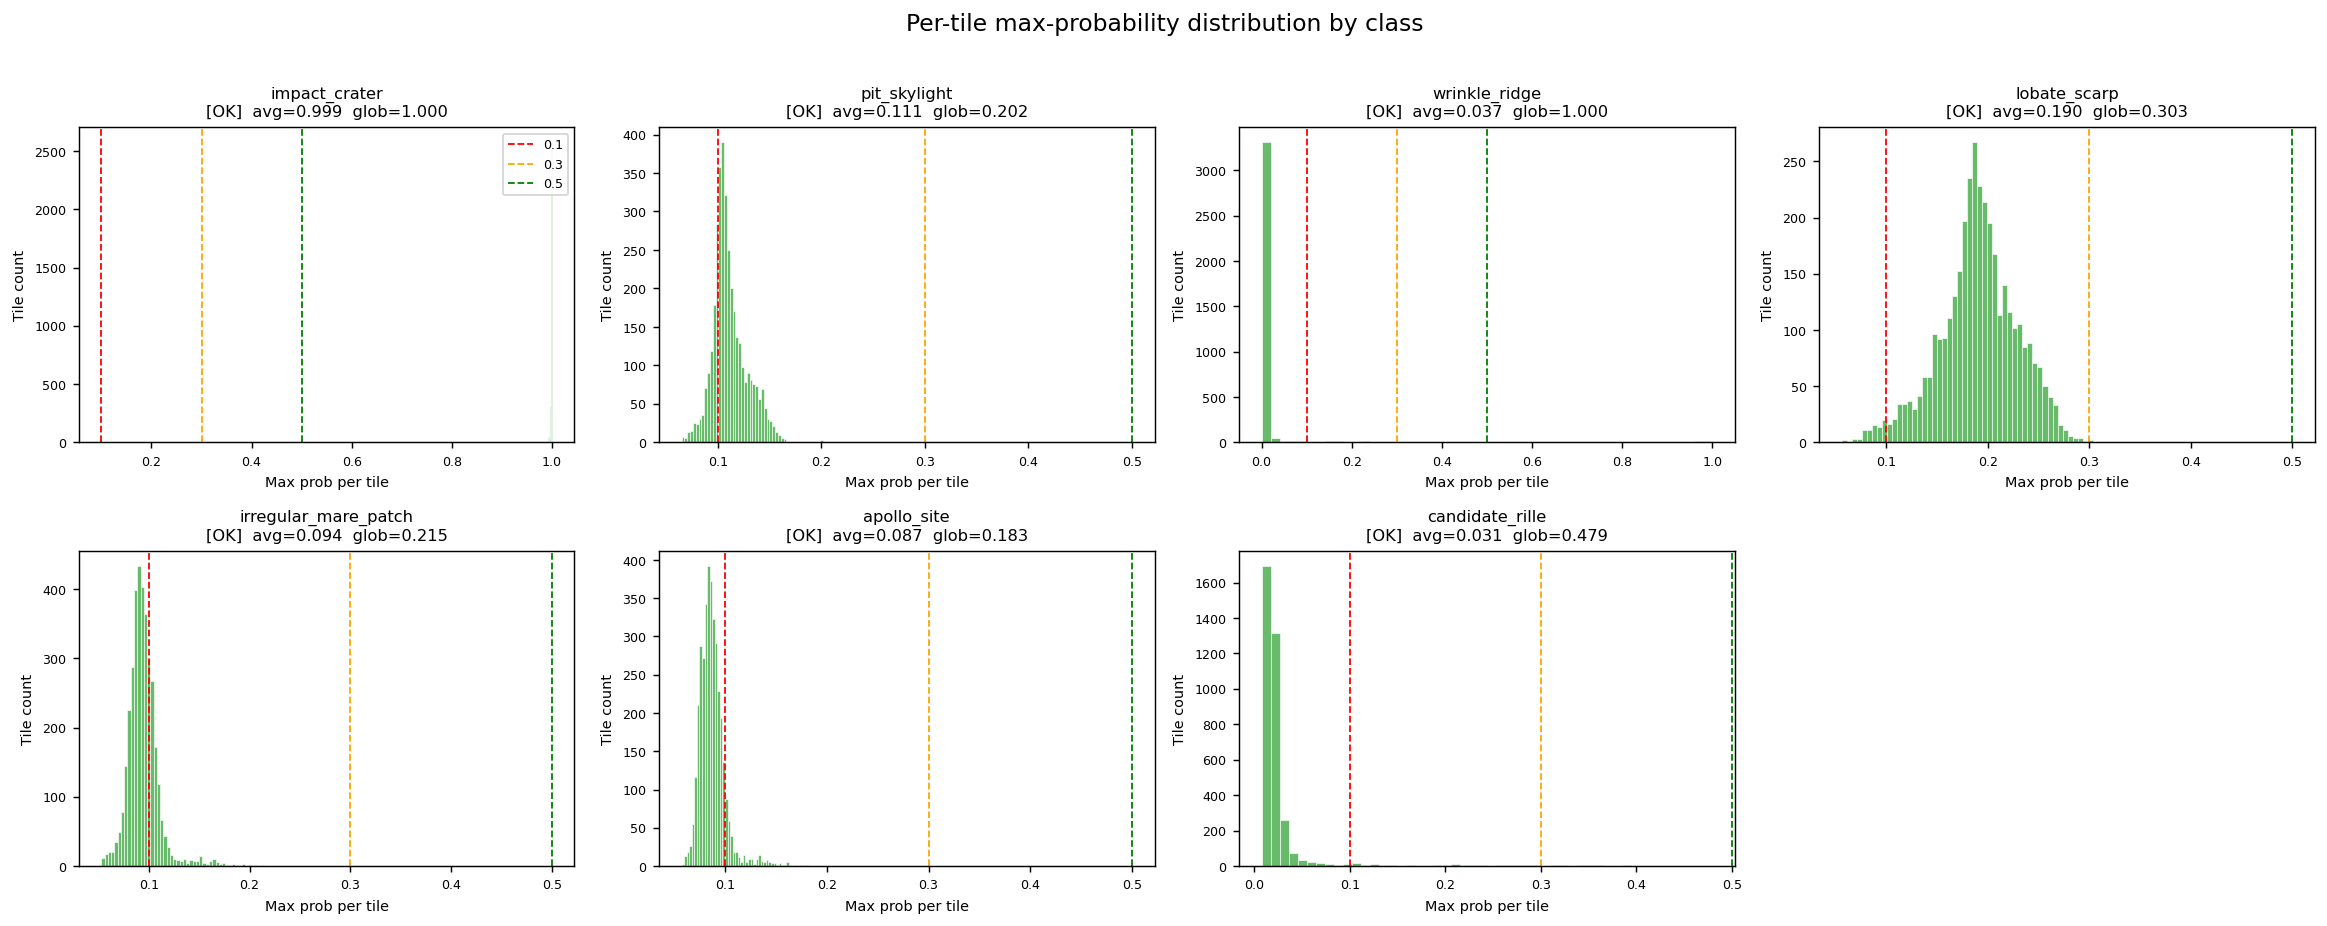
\includegraphics[width=\textwidth]{figures/MR/diagnostics_distributions.png}
    \caption{Per-tile max-probability distributions.}
\end{subfigure}
\hfill
\begin{subfigure}[b]{0.48\textwidth}
    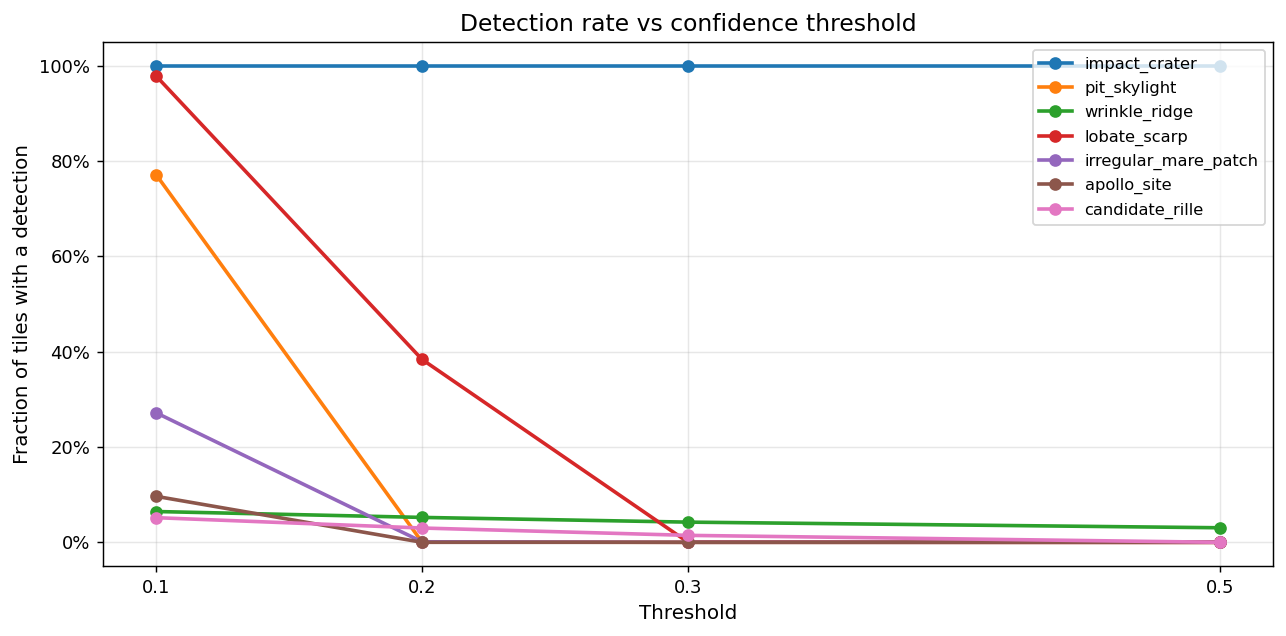
\includegraphics[width=\textwidth]{figures/MR/diagnostics_detection_rates.png}
    \caption{Detection rate vs.\ confidence threshold.}
\end{subfigure}
\caption{South pole inference diagnostics across 3\,639 tiles. Impact craters are detected with near-certainty across the entire region. All other classes exhibit strongly right-skewed distributions with low average confidence, reflecting both the domain shift from Marius Hills and the scarcity of these features at the south pole.}
\label{fig:south_pole_diag}
\end{figure}

\begin{figure}[htbp!]
\centering
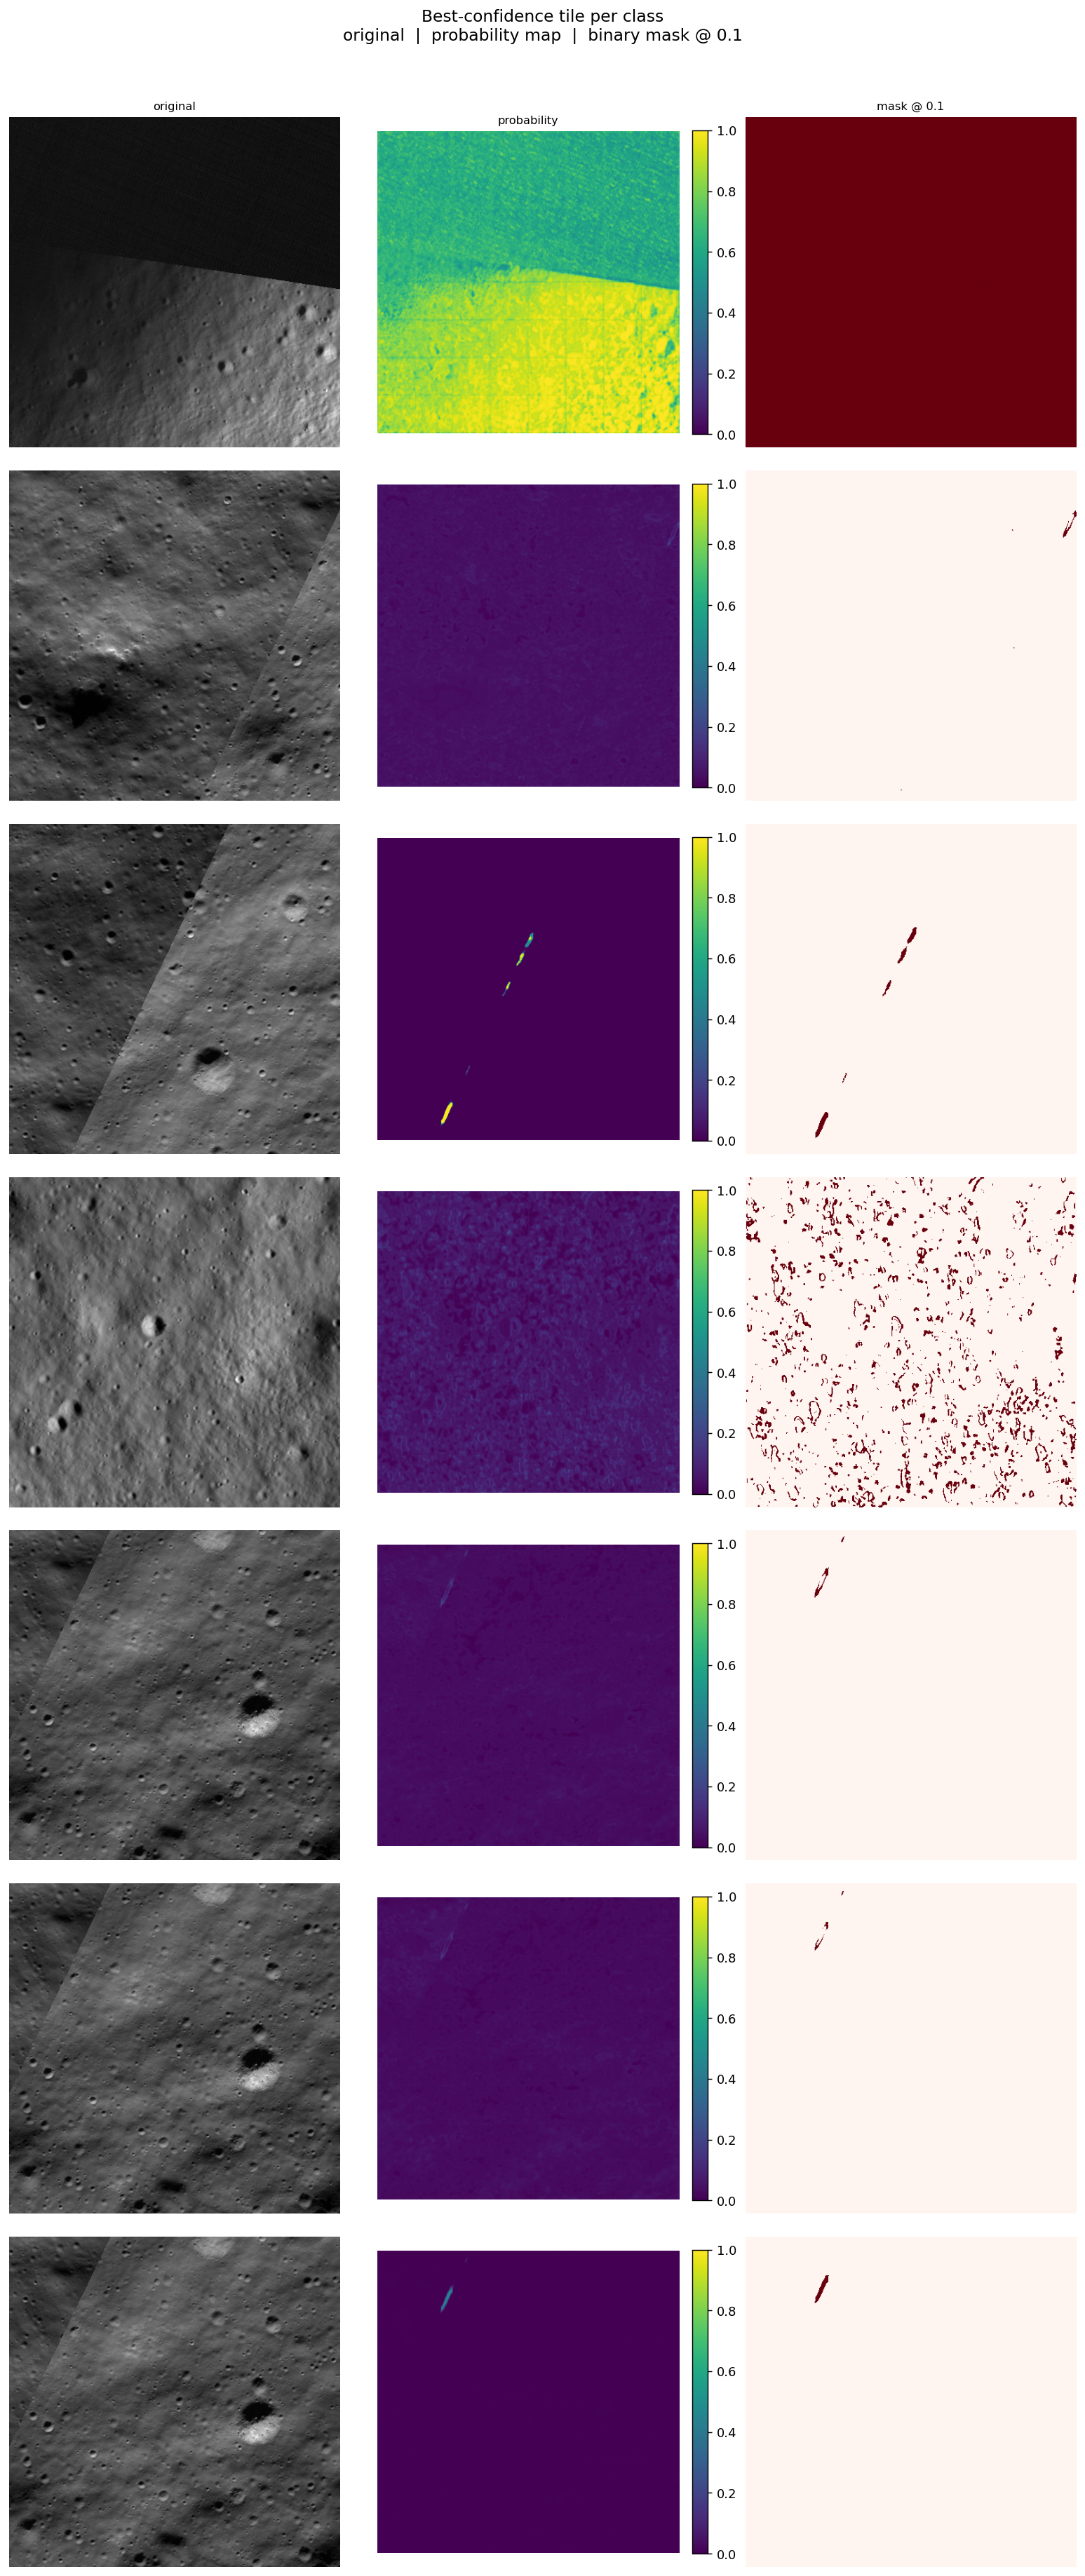
\includegraphics[width=0.85\columnwidth,keepaspectratio]{figures/MR/diagnostics_best_tiles.png}
\caption{Best-detected tile per class on the south pole imagery. Each panel shows the LRO WAC tile overlaid with the predicted probability map for the class with the highest maximum confidence in that tile. Overlays use a \emph{relative} threshold (top fraction of each tile's probabilities) so that the most likely candidate pixels are visible even when absolute confidence is low; coloured regions for the weak classes are therefore candidate locations, not confident detections.}
\label{fig:south_pole_best}
\end{figure}

The model assigns high crater probability across the entire south pole (average max probability 0.863). Given the near-saturated crater layer learned in training (Sect.~\ref{sec:mr_dataset}) --- and the base-rate analysis of Sect.~\ref{sec:comp_crater} --- this is expected behaviour and should not be over-interpreted as precise crater delineation. Two classes, \texttt{wrinkle\_ridge} and \texttt{candidate\_rille}, show very low average-tile probabilities but anomalously high global maxima (1.000 and 0.480): the model makes rare but confident predictions on a small number of tiles rather than diffuse activations everywhere. The weak performance on rare classes is attributable to the combination of domain shift (the south pole lacks the volcanic structures that dominate the training distribution) and the near-absence of supervision for those classes even in the training region.

\subsection{Scaling the inference pipeline, and a reproducibility lesson}
\label{sec:sp_pipeline}

Running the segmentation transfer at survey scale required dedicated engineering: a decoupled inference pipeline that streams tiles through the network, serialises each probability cube immediately to compressed \texttt{.npz} storage in a directory split from the visual outputs (preventing RAM exhaustion over thousands of tiles), and aggregates statistics in a second pass over the stored arrays into a central \texttt{stats.json} catalogue. This architecture processed the full tile set without runtime failures and is the backbone of Table~\ref{tab:south_pole_stats}.

An early run of this pipeline, however, produced results that contradicted Table~\ref{tab:south_pole_stats}: every class, including the five with essentially no supervision, appeared with average maximum probabilities in a narrow band around 0.5 and identical detection counts of $262\,144$ ($=512^2$) pixels per tile; the corresponding visual outputs (Fig.~\ref{fig:mega_grid_3x2}) show flat, structureless probability fields on every class. Diagnosing this discrepancy proved instructive. The checkpoint had been saved by an earlier revision of the architecture whose layer names differed; loading it with non-strict key matching silently matched \emph{zero} convolutional layers, so the network ran with its random initialisation --- producing sigmoid outputs clustered around $0.5$ everywhere, exactly as observed. A second, independent mismatch compounded it: the tile loader re-implemented CLAHE with different parameters (OpenCV, clip limit 2.0) than the training pipeline (\texttt{skimage}, clip limit 0.03), feeding the network inputs from a different distribution than it was trained on. Both defects are now fixed in the shared codebase (checkpoint keys are remapped explicitly and loading surfaces any mismatch; preprocessing is imported from the training package rather than re-implemented), and a re-run of the corrected pipeline on a 300-tile sample reproduces the reference behaviour of Table~\ref{tab:south_pole_stats}: crater-dominant near-saturated confidence, all rare classes weak, and the characteristic rare-but-confident maxima of the ridge and rille channels --- in place of the uniform $\approx 0.5$ signature of the defective run. We report this because it is a textbook failure mode of multi-author deep-learning projects: non-strict checkpoint loading turns an interface mismatch into silently plausible-looking numbers, and only the cross-check against an independent run of the same model exposed it.

\begin{figure*}[htbp]
\centering
  \begin{subfigure}[b]{0.4\textwidth}
    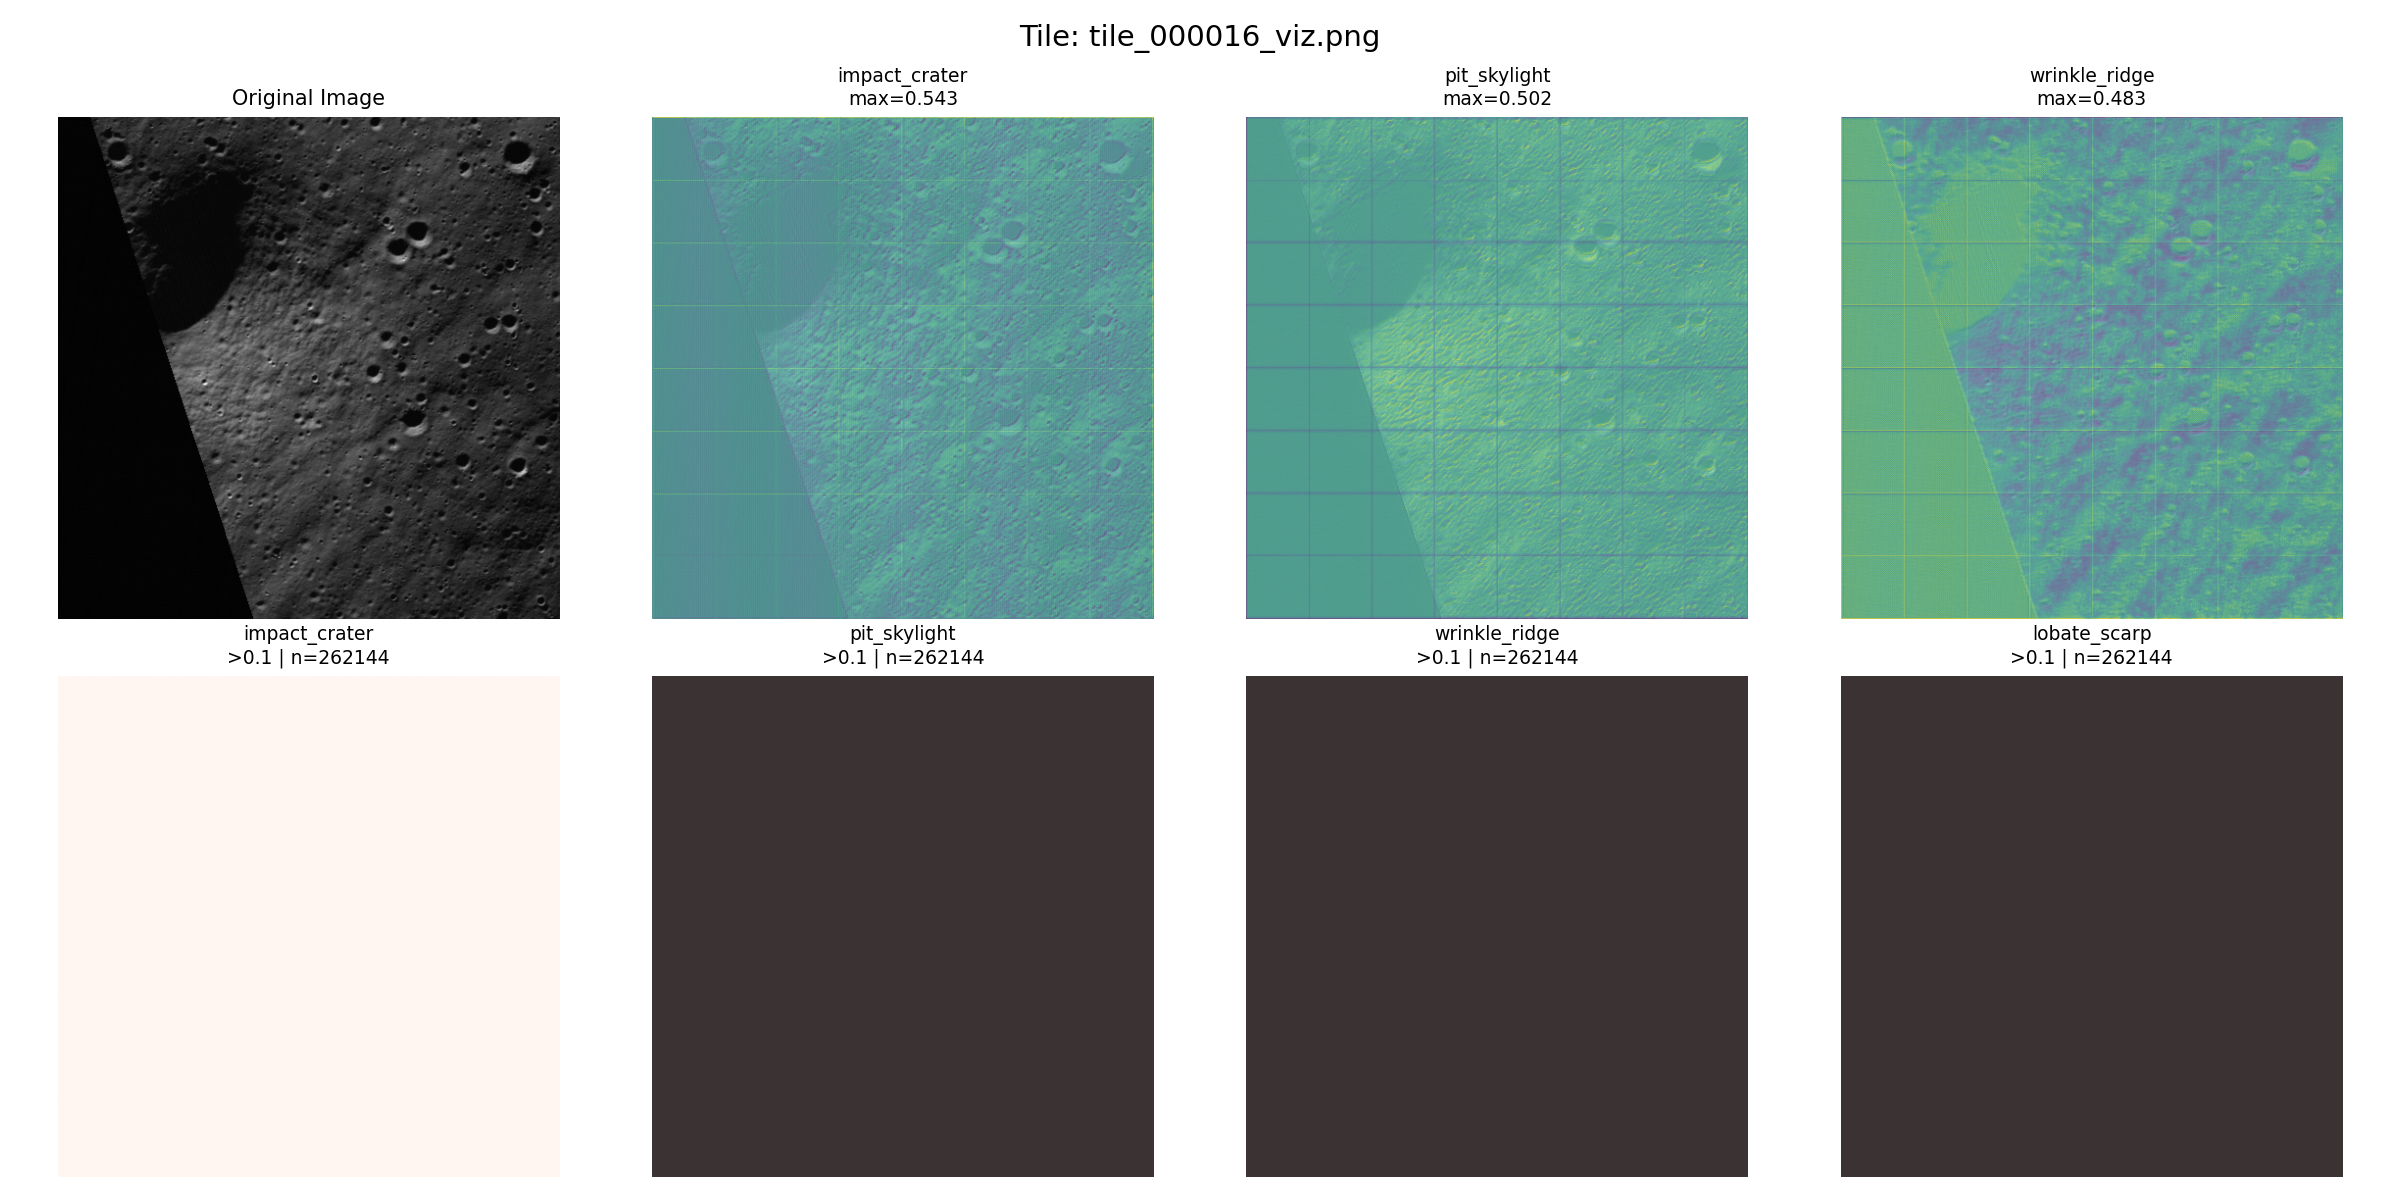
\includegraphics[width=\textwidth]{output1.png}
    \caption{Tile 1.}
  \end{subfigure}
  \hfill
  \begin{subfigure}[b]{0.4\textwidth}
    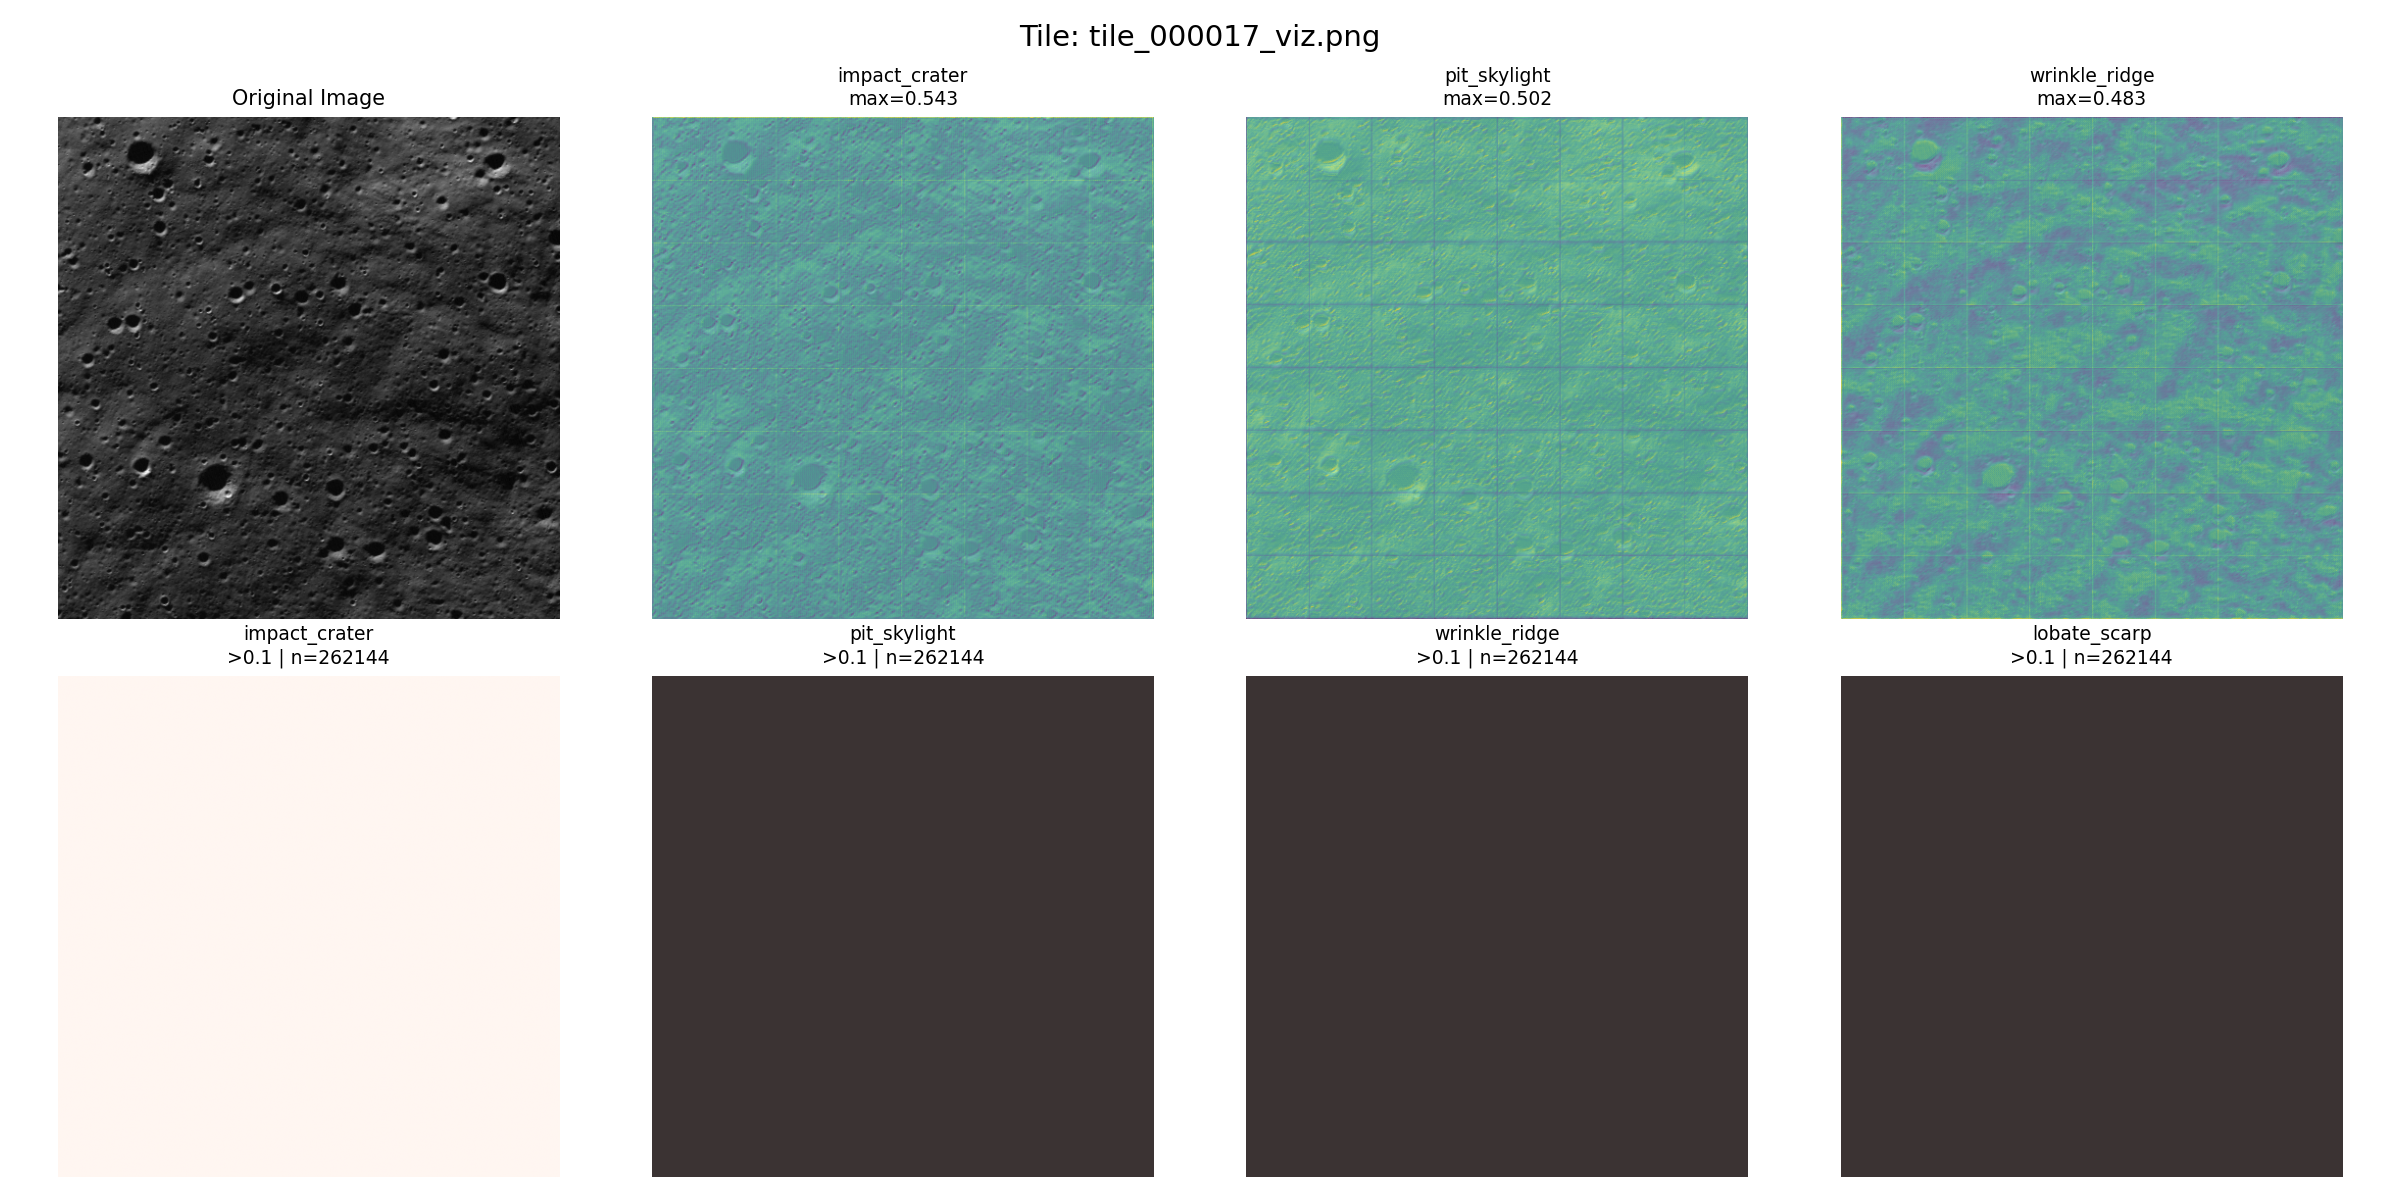
\includegraphics[width=\textwidth]{output2.png}
    \caption{Tile 2.}
  \end{subfigure}
  \hfill
  \begin{subfigure}[b]{0.4\textwidth}
    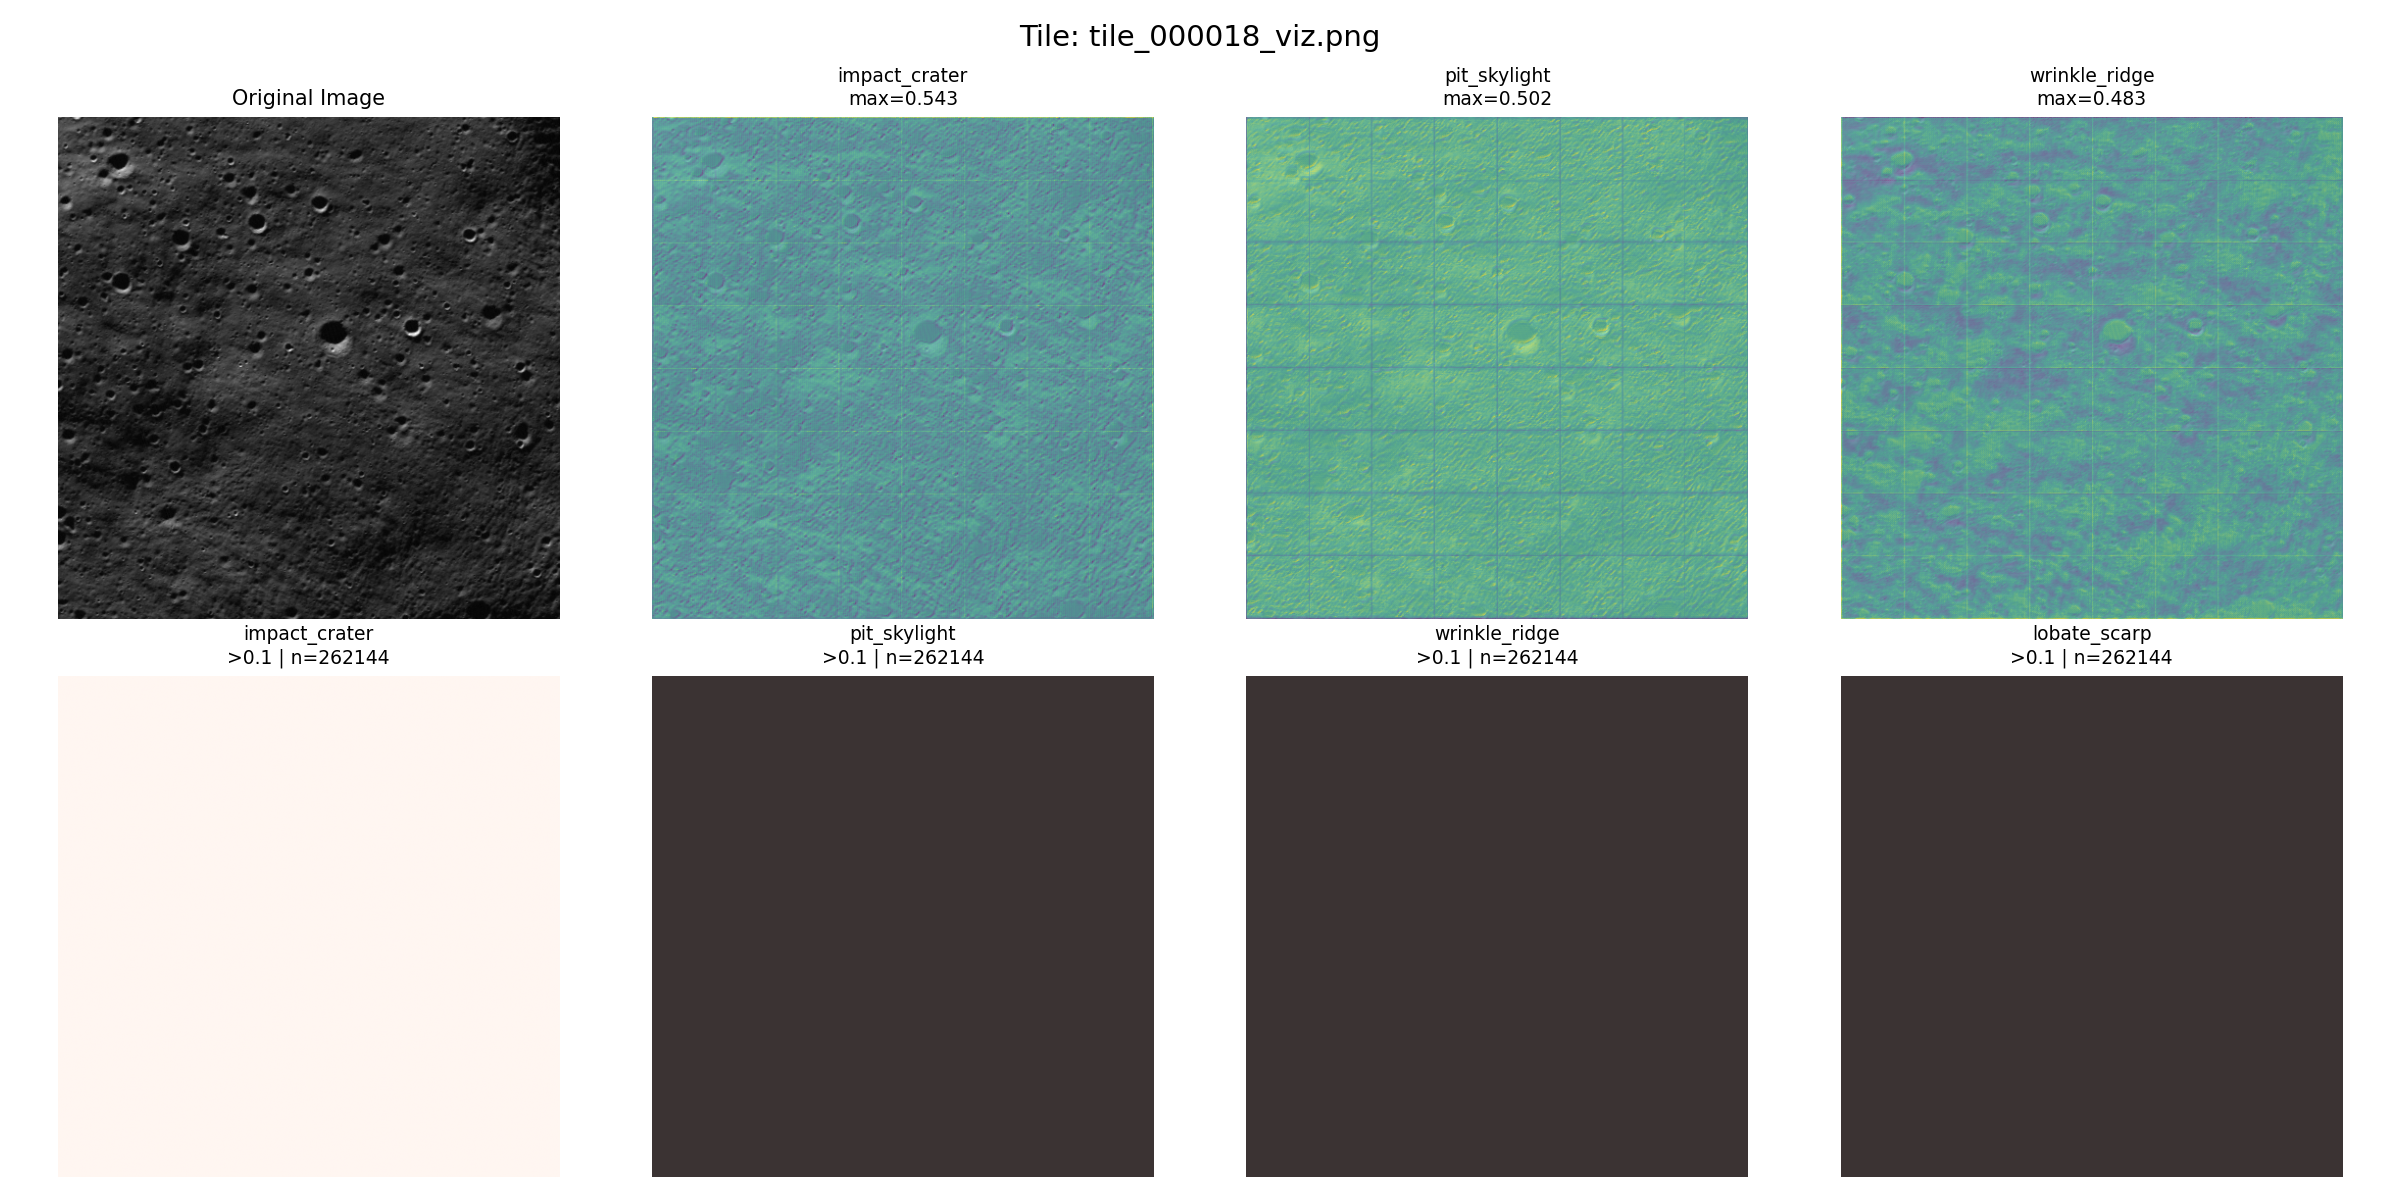
\includegraphics[width=\textwidth]{output3.png}
    \caption{Tile 3.}
  \end{subfigure}

  \vspace{0.5cm}
  \begin{subfigure}[b]{0.4\textwidth}
    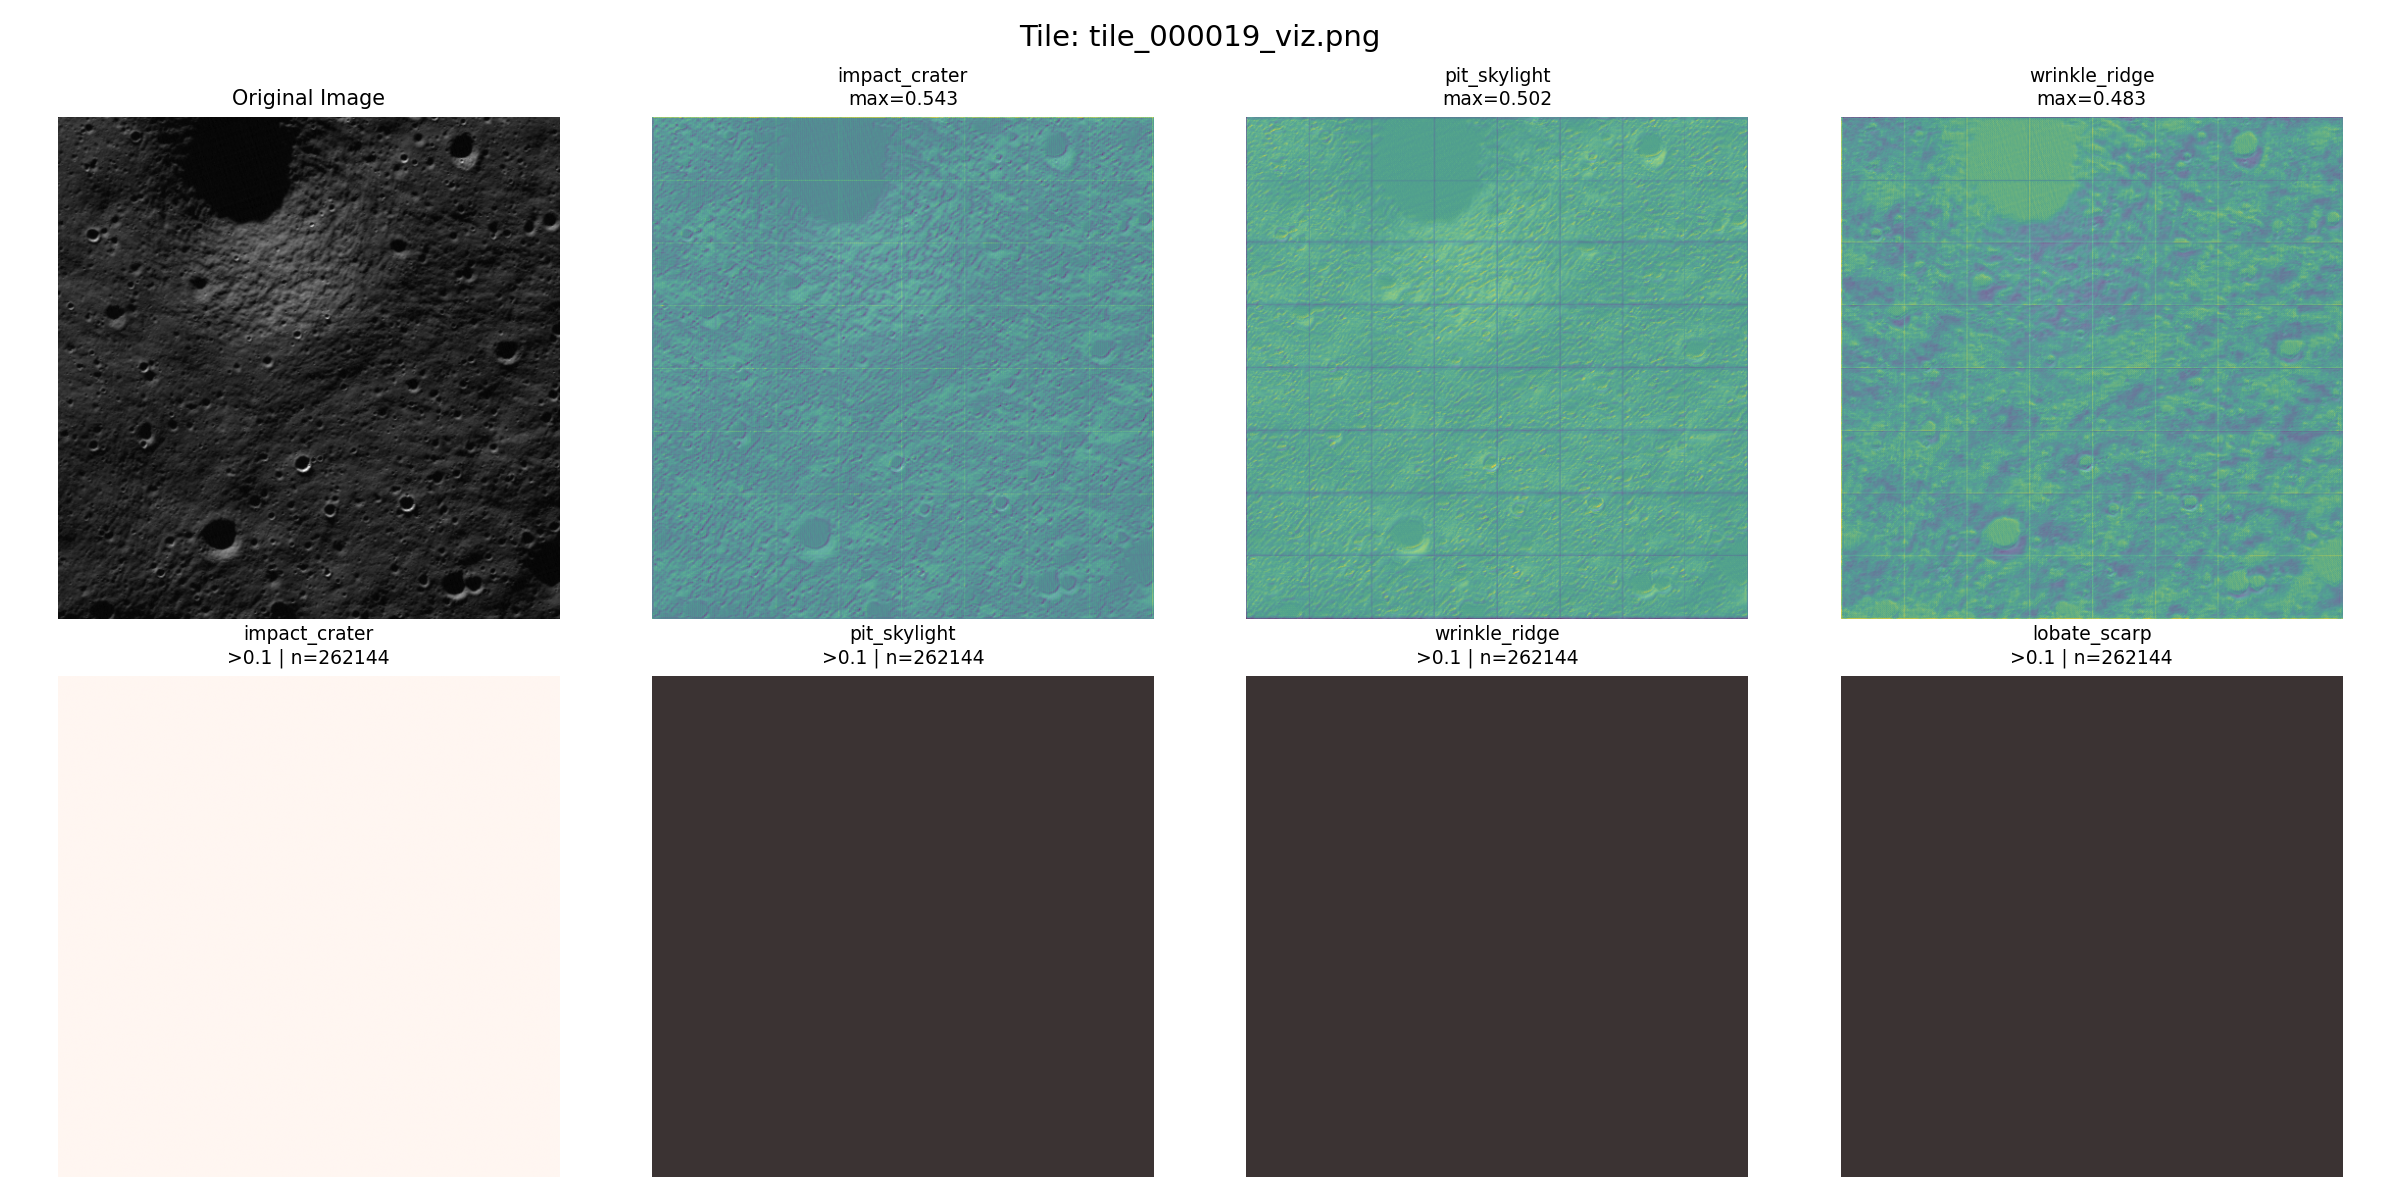
\includegraphics[width=\textwidth]{output4.png}
    \caption{Tile 4.}
  \end{subfigure}
  \hfill
  \begin{subfigure}[b]{0.4\textwidth}
    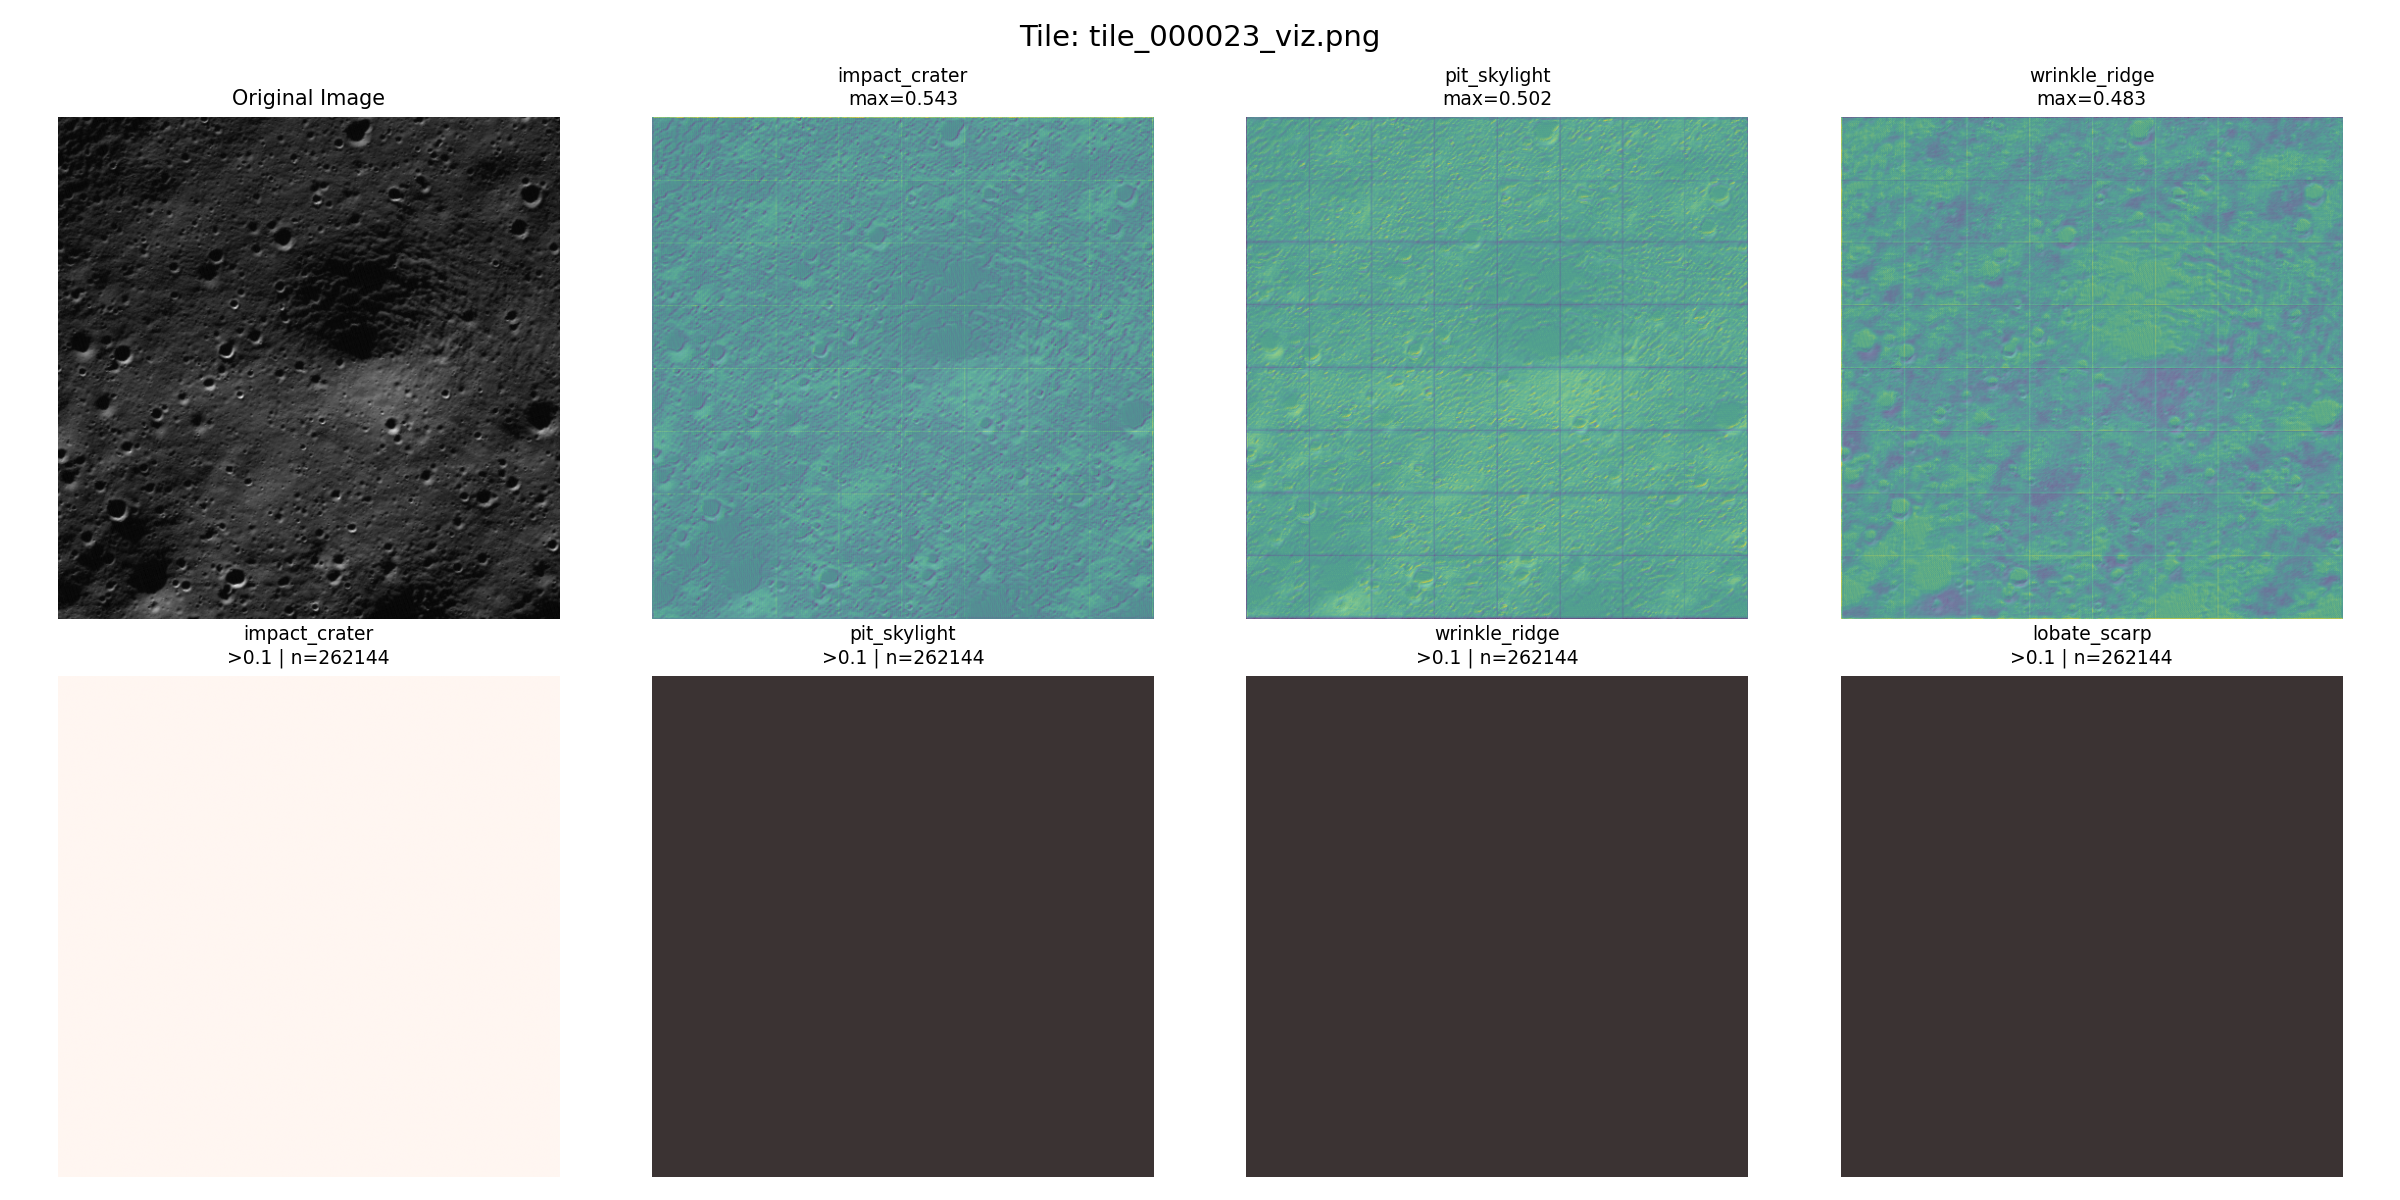
\includegraphics[width=\textwidth]{output5.png}
    \caption{Tile 5.}
  \end{subfigure}
  \hfill
  \begin{subfigure}[b]{0.4\textwidth}
    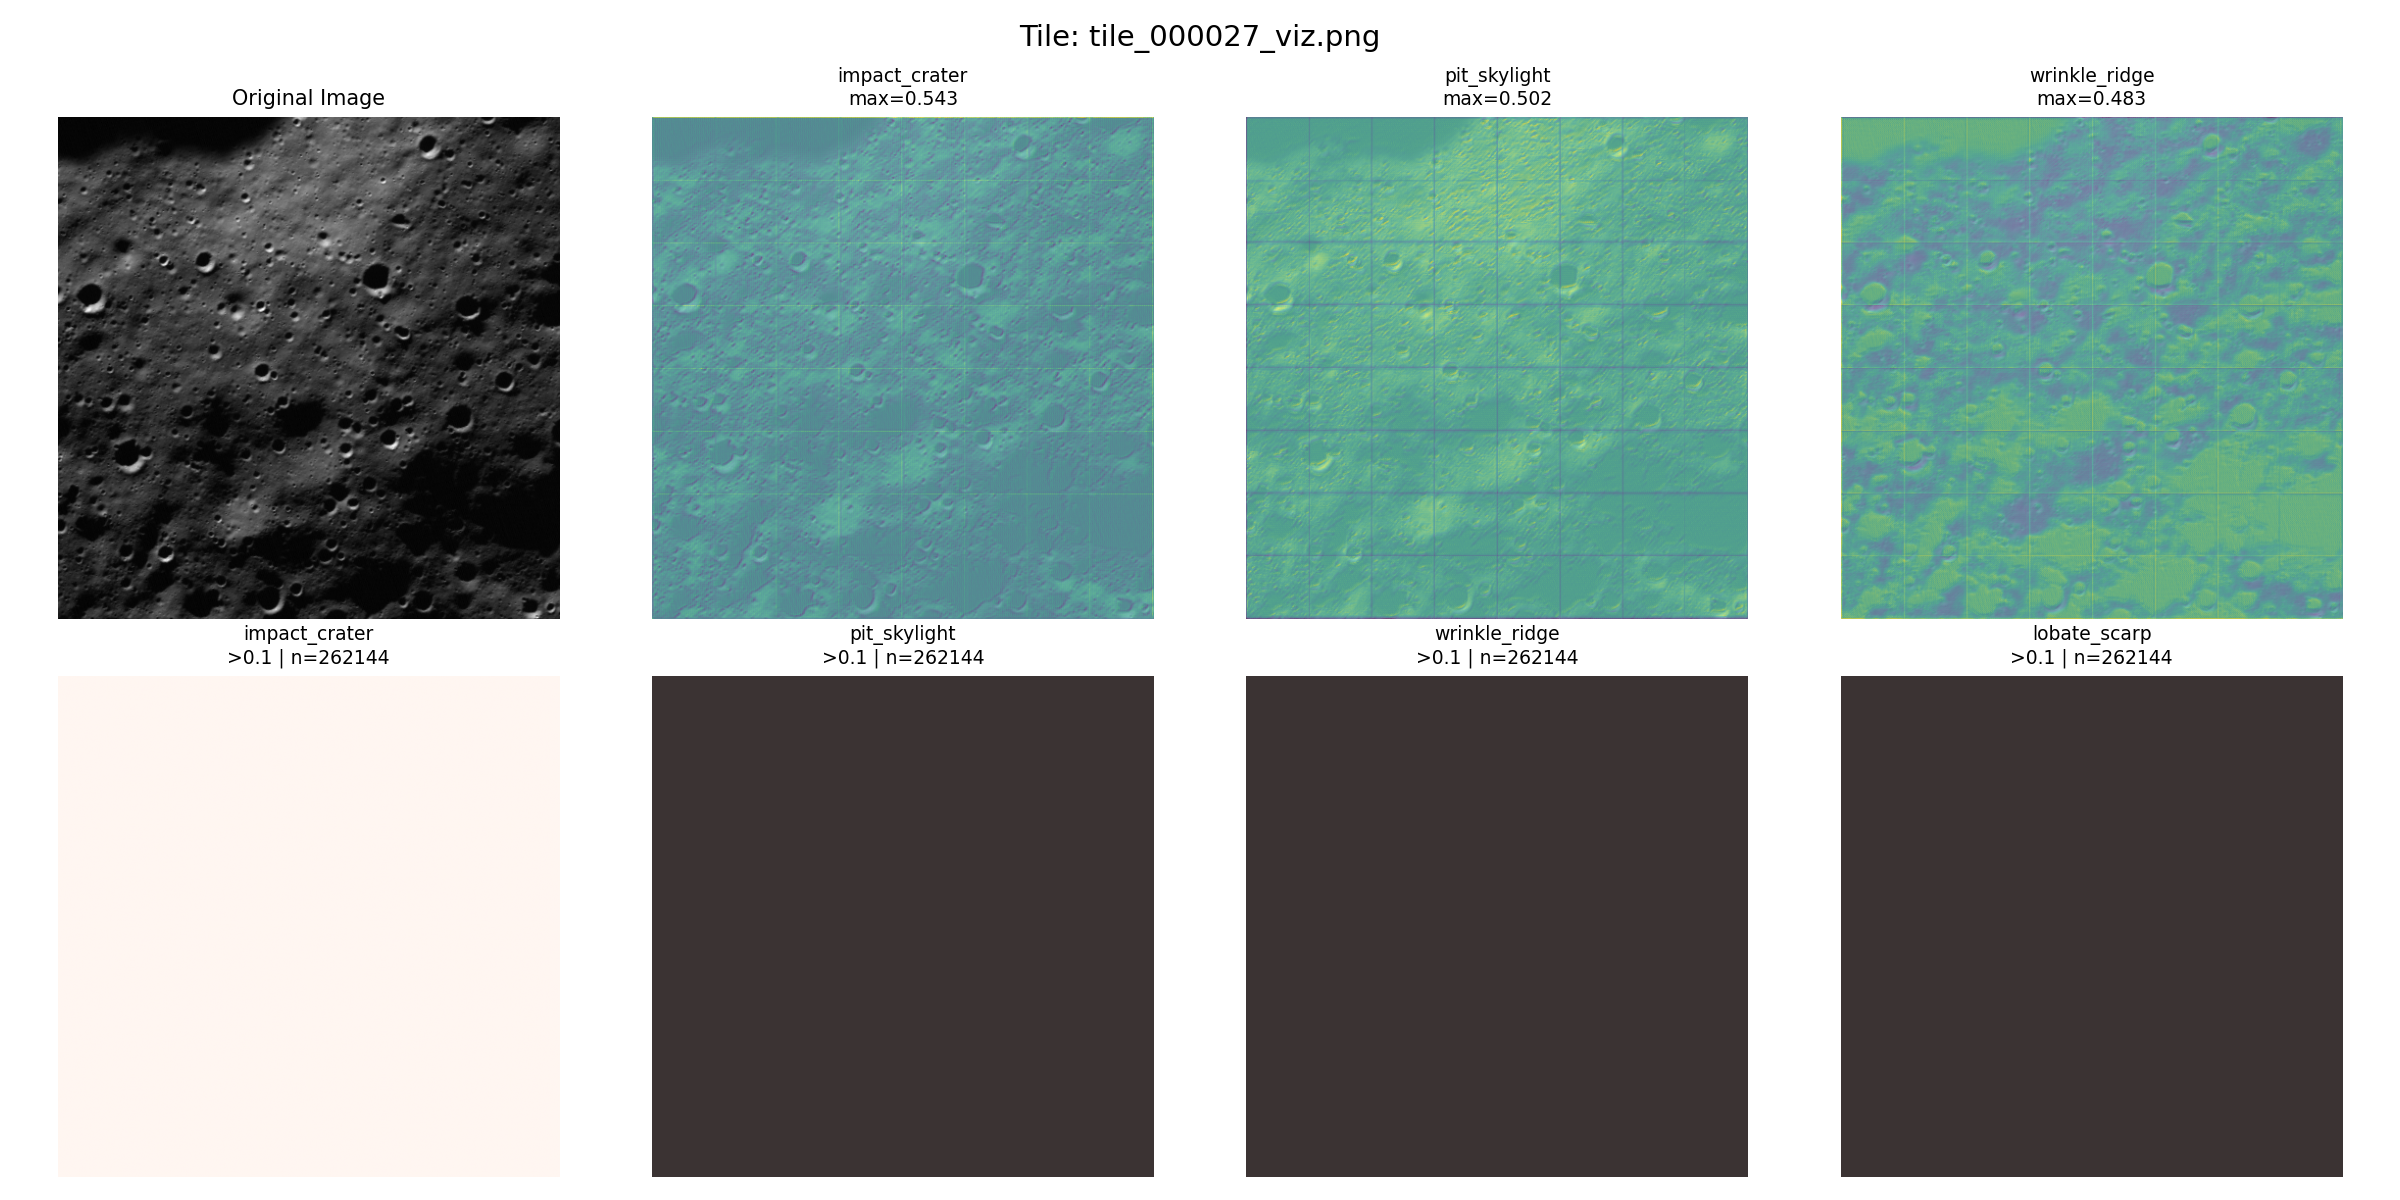
\includegraphics[width=\textwidth]{output6.png}
    \caption{Tile 6.}
  \end{subfigure}

\caption{Visual-verification outputs of the \emph{initial, defective} pipeline run on six south pole tiles (original imagery alongside per-class probability overlays). The overlays are flat and near-uniform regardless of the underlying morphology --- the visual signature of the silently unmatched checkpoint described in the text: a randomly initialised network outputs $\approx 0.5$ everywhere, which post-processing renders as structureless fields. The corrected pipeline instead reproduces the class-selective behaviour of Table~\ref{tab:south_pole_stats}. The panels are retained precisely because they show how plausible a defective run can look at a glance.}
\label{fig:mega_grid_3x2}
\end{figure*}

\subsection{Detection-level transfer: YOLOv8 and Mask R-CNN}
\label{sec:sp_yolo}

The two detection formulations were likewise deployed on the same tiles, and their disagreement is as instructive as their agreement.

The YOLOv8 ensemble of Sect.~\ref{sec:yolo_ensemble}, at a confidence threshold of $\geq 0.5$, predicts a feature population that is overwhelmingly craters (98.0\% of detections), followed by wrinkle ridges (1.4\%) and lobate scarps (0.6\%) --- a plausible composition for heavily cratered highland terrain, consistent with the crater-dominant segmentation diagnostics above and with the tectonic (contraction-driven) origin of the ridge and scarp detections.

The Mask R-CNN of Sect.~\ref{sec:maskrcnn}, evaluated at its own operating threshold (0.5) on all 3\,639 tiles, tells a different story: it returns only 52 instances in the entire region, \emph{all} classified as wrinkle ridges, and \emph{zero} craters. Craters emerge only when the confidence threshold is lowered --- 188 detections on 78 tiles at $\tau = 0.2$, 8\,176 at $\tau = 0.1$, and 104\,871 at $\tau = 0.05$. This is the domain-shift signature of a detector whose crater recall was already its weak point in-distribution (Sect.~\ref{sec:maskrcnn}): on unfamiliar terrain its crater confidence collapses below the nominal operating point while its ridge head remains assertive. The lesson mirrors the threshold-calibration requirement of the shared protocol (Sect.~\ref{sec:metrics_protocol}), now in a regime where no calibration set exists.

With no ground truth, none of these compositions can be validated individually. Read together, the three formulations triangulate what a single pipeline cannot: the segmentation diagnostics and YOLOv8 agree that the region is crater-dominated with rare linear tectonic features, while Mask R-CNN's threshold sweep shows how strongly any such composition depends on confidence calibration under domain shift. In an unlabelled region, cross-method comparison is not just the best available check --- it is also the only way to see which conclusions are threshold-robust and which are not.
